\documentclass[aspectratio=169]{beamer}

% Theme and Color
\usetheme{Madrid}
\usecolortheme{whale}

% Packages
\usepackage{graphicx}
\usepackage{amsmath}
\usepackage{amssymb}
\usepackage{siunitx}
\usepackage{booktabs}
\usepackage{tikz}
\usetikzlibrary{Octorations.pathmorphing}
\usepackage{multirow}

% Custom colors
\definecolor{mitblue}{RGB}{0,51,102}
\definecolor{mitred}{RGB}{204,0,0}
\setbeamercolor{structure}{fg=mitblue}
\setbeamercolor{title}{fg=white,bg=mitblue}
\setbeamercolor{frametitle}{fg=white,bg=mitblue}

% Remove navigation symbols
\setbeamertemplate{navigation symbols}{}

% Footer
\setbeamertemplate{footline}{
  \leavevmode%
  \hbox{%
  \begin{beamercolorbox}[wd=.333333\paperwidth,ht=2.25ex,dp=1ex,center]{author in head/foot}%
    \usebeamerfont{author in head/foot}\insertshortauthor
  \end{beamercolorbox}%
  \begin{beamercolorbox}[wd=.333333\paperwidth,ht=2.25ex,dp=1ex,center]{title in head/foot}%
    \usebeamerfont{title in head/foot}\insertshorttitle
  \end{beamercolorbox}%
  \begin{beamercolorbox}[wd=.333333\paperwidth,ht=2.25ex,dp=1ex,right]{date in head/foot}%
    \usebeamerfont{date in head/foot}\insertshortdate{}\hspace*{2em}
    \insertframenumber{} / \inserttotalframenumber\hspace*{2ex} 
  \end{beamercolorbox}}%
  \vskip0pt%
}

% Title page info
\title[Active Suspension System]{Active Suspension System}
\subtitle{Design and Performance Analysis}
\author[Manikanta \& Rounak]{
    Gonugondla Veera Manikanta (230906450) \\
    Rounak Pradhan (230906492)
}
\institute[MIT]{
    Department of Electrical \& Electronics Engineering \\
    Manipal Institute of Technology, Manipal - 576104
}
\date[Oct 2025]{Systems Simulation Laboratory (ELE 3142) \\ October 2025}

\begin{document}

% Title Slide
\begin{frame}
  \titlepage
\end{frame}

% Outline
\begin{frame}{Outline}
  \tableofcontents
\end{frame}

% Section 1: Introduction
\section{Introduction}

\begin{frame}{What's the Problem?}
  \begin{columns}
    \column{0.5\textwidth}
    \textbf{Why Passive Suspension Isn't Great:}
    \begin{itemize}
      \item Springs and dampers are fixed - can't adapt
      \item You have to choose: comfort OR handling
      \item Bad at dealing with different road conditions
      \item Takes forever to stop bouncing
      \item No way to optimize performance
    \end{itemize}
    
    \column{0.5\textwidth}
    \begin{center}
      \begin{tikzpicture}[scale=0.7]
        % Simple car illustration
        \draw[fill=gray!30] (0,0) rectangle (4,0.5);
        \draw[fill=gray!50] (0.5,0.5) rectangle (3.5,1.5);
        \draw[thick] (1,0) -- (1,-0.5) -- (1,-1);
        \draw[thick] (3,0) -- (3,-0.5) -- (3,-1);
        \draw[thick,Octoration={coil,aspect=0.3,segment length=3mm},Octorate] (1,-0.5) -- (1,-1);
        \draw[thick,Octoration={coil,aspect=0.3,segment length=3mm},Octorate] (3,-0.5) -- (3,-1);
        \draw[fill=black] (1,-1.3) circle (0.3);
        \draw[fill=black] (3,-1.3) circle (0.3);
        \draw[thick] (0,-1.6) -- (4,-1.6);
        \node at (2,2) {\textbf{Passive Suspension}};
      \end{tikzpicture}
    \end{center}
  \end{columns}
\end{frame}

\begin{frame}{Why We Did This Project}
  \begin{block}{Our Motivation}
    \begin{itemize}
      \item We wanted to see if we could make suspension better using control systems
      \item Active suspension can adapt in real-time to what's happening
      \item Should reduce vibrations and make the ride smoother
      \item Improve both comfort AND handling at the same time
    \end{itemize}
  \end{block}
  
  \vspace{0.3cm}
  
  \begin{block}{What We Set Out to Do}
    \begin{enumerate}
      \item Build a mathematical model of the suspension system
      \item Design a PID controller to actively control it
      \item Simulate everything in MATLAB/Simulink
      \item Compare how well passive vs active performs
      \item Analyze the results in frequency and time domains
    \end{enumerate}
  \end{block}
\end{frame}

% Section 2: System Modeling
\section{Our System Model}

\begin{frame}{The Quarter-Car Model We Used}
  \begin{columns}
    \column{0.45\textwidth}
    \textbf{What's in our model:}
    \begin{itemize}
      \item $m_s$: Car body mass
      \item $m_{us}$: Wheel mass
      \item $k_s$: Suspension spring
      \item $c_s$: Suspension damper
      \item $k_t$: Tire spring
      \item $c_t$: Tire damper
      \item $F_c$: Our control force
    \end{itemize}
    
    \column{0.55\textwidth}
    \begin{center}
      \begin{tikzpicture}[scale=0.85]
        % Body mass (sprung mass)
        \draw[fill=blue!30,thick,rounded corners=2pt] (-0.8,5) rectangle (0.8,5.8);
        \node[font=\large] at (0,5.4) {$m_s$};
        
        % Suspension spring
        \draw[thick,Octoration={coil,aspect=0.3,segment length=2.5mm,amplitude=4mm},Octorate] 
          (-0.4,3.8) -- (-0.4,5);
        \node[left,font=\small] at (-0.5,4.4) {$k_s$};
        
        % Suspension damper
        \draw[thick] (0.4,3.8) -- (0.4,4.2);
        \draw[thick,fill=white] (0.2,4.2) rectangle (0.6,4.7);
        \draw[thick] (0.4,4.7) -- (0.4,5);
        \draw[thick] (0.15,4.35) -- (0.65,4.35);
        \draw[thick] (0.15,4.55) -- (0.65,4.55);
        \node[right,font=\small] at (0.7,4.45) {$c_s$};
        
        % Wheel mass (unsprung mass)
        \draw[fill=orange!30,thick,rounded corners=2pt] (-0.6,2.8) rectangle (0.6,3.8);
        \node[font=\large] at (0,3.3) {$m_{us}$};
        
        % Tire spring
        \draw[thick,Octoration={coil,aspect=0.3,segment length=2mm,amplitude=3mm},Octorate] 
          (-0.35,1.2) -- (-0.35,2.8);
        \node[left,font=\small] at (-0.45,2) {$k_t$};
        
        % Tire damper
        \draw[thick] (0.35,1.2) -- (0.35,1.6);
        \draw[thick,fill=white] (0.2,1.6) rectangle (0.5,2.1);
        \draw[thick] (0.35,2.1) -- (0.35,2.8);
        \draw[thick] (0.15,1.75) -- (0.55,1.75);
        \draw[thick] (0.15,1.95) -- (0.55,1.95);
        \node[right,font=\small] at (0.55,1.85) {$c_t$};
        
        % Road surface
        \fill[pattern=north east lines] (-1.5,1) rectangle (1.5,1.2);
        \draw[very thick] (-1.5,1.2) -- (1.5,1.2);
        \node[below,font=\small] at (0,0.9) {Road: $x_r$};
        
        % Control force arrow
        \draw[->,ultra thick,red!70!black] (1.2,5.4) -- (2,5.4);
        \node[right,red!70!black,font=\small] at (2,5.4) {$F_c$};
        
        % Displacement arrows
        \draw[<->,thick,blue] (-1.3,5.4) -- (-1.3,3.3);
        \node[left,blue,font=\footnotesize] at (-1.3,4.35) {$x_s$};
        
        \draw[<->,thick,orange] (-1.3,3.3) -- (-1.3,1.2);
        \node[left,orange,font=\footnotesize] at (-1.3,2.25) {$x_{us}$};
      \end{tikzpicture}
    \end{center}
  \end{columns}
\end{frame}

\begin{frame}{Parameters We Used}
  \begin{table}
    \centering
    \begin{tabular}{lcc}
      \toprule
      \textbf{Parameter} & \textbf{Value} & \textbf{Unit} \\
      \midrule
      Car body mass, $m_s$ & 300 & kg \\
      Wheel mass, $m_{us}$ & 40 & kg \\
      Suspension spring, $k_s$ & 18,000 & N/m \\
      Suspension damping, $c_s$ & 1,200 & N·s/m \\
      Tire stiffness, $k_t$ & 195,000 & N/m \\
      Tire damping, $c_t$ & 75 & N·s/m \\
      \bottomrule
    \end{tabular}
  \end{table}
  
  \vspace{0.5cm}
  
  \textbf{Note:} We got these values from typical passenger car specifications
\end{frame}

\begin{frame}{Equations of Motion}
  We applied Newton's second law to both masses:
  
  \begin{block}{For the car body:}
    \vspace{-0.2cm}
    \begin{equation}
      m_s \ddot{x}_s = -k_s(x_s - x_{us}) - c_s(\dot{x}_s - \dot{x}_{us}) + F_c
    \end{equation}
  \end{block}
  
  \begin{block}{For the wheel:}
    \vspace{-0.2cm}
    \begin{equation}
      \begin{split}
      m_{us} \ddot{x}_{us} = k_s(x_s - x_{us}) + c_s(\dot{x}_s - \dot{x}_{us}) \\
      - k_t(x_{us} - x_r) - c_t(\dot{x}_{us} - \dot{x}_r) - F_c
      \end{split}
    \end{equation}
  \end{block}
  
  These describe how forces affect the motion of each mass.
\end{frame}

% Section: Transfer Function
\section{Transfer Function Derivation}

\begin{frame}{Getting the Transfer Function}
  \textbf{Step 1: We took the Laplace Transform}
  
  \small
  \begin{align}
    m_s s^2 X_s &= -(c_s s + k_s)(X_s - X_{us}) + F_c \\
    m_{us} s^2 X_{us} &= (c_s s + k_s)(X_s - X_{us}) \nonumber \\
    &\quad - (c_t s + k_t)(X_{us} - X_r) - F_c
  \end{align}
  
  \normalsize
  \vspace{0.3cm}
  
  \textbf{Step 2: For passive (no control), we eliminated $X_{us}$}
  
  \begin{block}{We got:}
    \vspace{-0.2cm}
    \begin{equation}
      G_p(s) = \frac{X_s(s)}{X_r(s)} = \frac{(c_s s + k_s)(c_t s + k_t)}{D(s)}
    \end{equation}
  \end{block}
\end{frame}

\begin{frame}{The Denominator Polynomial}
  \textbf{After doing all the algebra:}
  
  \small
  \begin{align}
    D(s) &= m_s m_{us} s^4 + (m_s c_t + m_{us} c_s)s^3 \nonumber \\
    &\quad + (m_s k_t + m_{us} k_s + c_s c_t)s^2 \nonumber \\
    &\quad + (c_s k_t + c_t k_s)s + k_s k_t
  \end{align}
  \normalsize
  
  \vspace{0.3cm}
  
  \textbf{What this tells us:}
  \begin{itemize}
    \item It's a 4th-order system (because of $s^4$)
    \item Natural frequency comes out to $\omega_n \approx 7.6$ rad/s (1.21 Hz)
    \item Damping ratio is $\zeta \approx 0.258$ (pretty underdamped!)
    \item All poles are stable (in left-half plane)
  \end{itemize}
\end{frame}

% Section: Controller Design
\section{Designing Our PID Controller}

\begin{frame}{Our Control Strategy}
  \begin{columns}
    \column{0.48\textwidth}
    \textbf{PID with a filter:}
    \begin{equation}
      C(s) = K_p + \frac{K_i}{s} + \frac{K_d N s}{s + N}
    \end{equation}
    
    \textbf{The gains we chose:}
    \begin{itemize}
      \item $K_p = 5000$
      \item $K_i = 100$
      \item $K_d = 2000$
      \item $N = 100$ (filter)
    \end{itemize}
    
    \textbf{Idea:} We feed back velocity and try to make it zero
    
    \column{0.52\textwidth}
    \begin{center}
      
    \end{center}
  \end{columns}
\end{frame}

\begin{frame}{How We Selected the Gains}
  \textbf{Here's our thought process:}
  
  \begin{enumerate}
    \item We calculated natural frequency: $\omega_n = 7.75$ rad/s
    
    \item We wanted damping ratio around 0.7 (critically damped)
    
    \item \textbf{Kp = 5000:} We made it about 28\% of the spring stiffness
    \begin{itemize}
      \item Not too high to cause instability
      \item Gives good response
    \end{itemize}
    
    \item \textbf{Kd = 2000:} About 40\% of Kp
    \begin{itemize}
      \item Acts like extra damping: $c_{eff} = 1200 + 2000 = 3200$ N·s/m
      \item This gives us $\zeta = 0.688$ - close to our target!
    \end{itemize}
    
    \item \textbf{Ki = 100:} Just 2\% of Kp
    \begin{itemize}
      \item Gets rid of steady-state error
      \item Small enough to avoid windup problems
    \end{itemize}
  \end{enumerate}
\end{frame}

\begin{frame}{Damping Ratio Improvement}
  \textbf{Passive system damping:}
  \begin{equation}
    \zeta_{passive} = \frac{c_s}{2\sqrt{k_s m_s}} = \frac{1200}{2\sqrt{18000 \times 300}} = 0.258
  \end{equation}
  
  \vspace{0.3cm}
  
  \textbf{With our controller (effective damping):}
  \begin{equation}
    \zeta_{active} = \frac{c_s + K_d}{2\sqrt{k_s m_s}} = \frac{3200}{2\sqrt{18000 \times 300}} = 0.688
  \end{equation}
  
  \vspace{0.5cm}
  
  \begin{alertblock}{That's a huge improvement!}
    \Large We increased damping by \textbf{166\%}!
  \end{alertblock}
\end{frame}

\begin{frame}{Stability Check}
  \textbf{We needed to make sure our system stays stable:}
  
  The closed-loop characteristic equation:
  \begin{equation}
    1 + C(s) \cdot s \cdot G_p(s) = 0
  \end{equation}
  
  \vspace{0.3cm}
  
  \textbf{Using Routh-Hurwitz criterion:}
  \begin{itemize}
    \item All coefficients turned out positive
    \item No sign changes in first column of Routh array
    \item This means all poles are in the left-half plane ✓
    \item Phase margin: $> 45°$ (good robustness)
    \item Gain margin: $> 6$ dB (also good)
  \end{itemize}
  
  \vspace{0.3cm}
  
  \textbf{Conclusion:} Our system is stable with good margins!
\end{frame}

% Section: Performance Calculations
\section{Calculating Performance}

\begin{frame}{Settling Time Calculation}
  For 2nd-order systems: $t_s = \frac{4}{\zeta \omega_n}$
  
  \vspace{0.3cm}
  
  \begin{columns}
    \column{0.5\textwidth}
    \textbf{Passive system:}
    \begin{equation}
      t_s = \frac{4}{0.258 \times 7.75} \approx 2.0 \text{ s}
    \end{equation}
    
    From simulation: 4.0 s
    
    (Higher because it's actually 4th-order)
    
    \column{0.5\textwidth}
    \textbf{Active system:}
    \begin{equation}
      t_s = \frac{4}{0.688 \times 7.75} \approx 0.75 \text{ s}
    \end{equation}
    
    From simulation: 1.5 s
    
    (Also 4th-order effect)
  \end{columns}
  
  \vspace{0.5cm}
  
  \begin{alertblock}{Result}
    \Large \textbf{62.5\% faster} settling!
  \end{alertblock}
\end{frame}

\begin{frame}{Overshoot Calculation}
  Formula: $\%OS = 100 \times e^{-\frac{\pi \zeta}{\sqrt{1-\zeta^2}}}$
  
  \vspace{0.3cm}
  
  \begin{columns}
    \column{0.5\textwidth}
    \textbf{Passive ($\zeta = 0.258$):}
    \begin{equation}
      \%OS = 43.6\%
    \end{equation}
    
    Pretty bouncy!
    
    \column{0.5\textwidth}
    \textbf{Active ($\zeta = 0.688$):}
    \begin{equation}
      \%OS = 4.3\%
    \end{equation}
    
    Much smoother!
  \end{columns}
  
  \vspace{0.5cm}
  
  \begin{alertblock}{Result}
    \Large \textbf{90\% less} overshoot
  \end{alertblock}
  
  \vspace{0.3cm}
  
  This means way smoother ride for passengers!
\end{frame}

\begin{frame}{Where the 15.24 dB Comes From}
  \textbf{At resonance frequency:}
  
  Magnitude amplification: $|G(j\omega_n)| = \frac{1}{2\zeta}$
  
  \vspace{0.3cm}
  
  \begin{columns}
    \column{0.5\textwidth}
    \textbf{Passive system:}
    \begin{align}
      |G_p| &= \frac{1}{2 \times 0.258} = 1.938 \\
      &= 5.75 \text{ dB}
    \end{align}
    
    We measured: 5.98 dB ✓
    
    \column{0.5\textwidth}
    \textbf{Active system:}
    \begin{align}
      |G_a| &= \frac{1}{2 \times 0.688} = 0.727 \\
      &= -2.77 \text{ dB}
    \end{align}
    
    We measured: -9.26 dB
  \end{columns}
  
  \vspace{0.4cm}
  
  \textbf{Difference:} $5.98 - (-9.26) = 15.24$ dB
  
  \textbf{In normal units:} $10^{15.24/20} = 5.77$× less vibration
  
  \textbf{Or:} \textbf{82.7\% reduction} in vibration amplitude!
\end{frame}

% Section: Simulation Results
\section{Our Simulation Results}

\begin{frame}{Simulink Model We Built}
  \begin{figure}
    \centering
    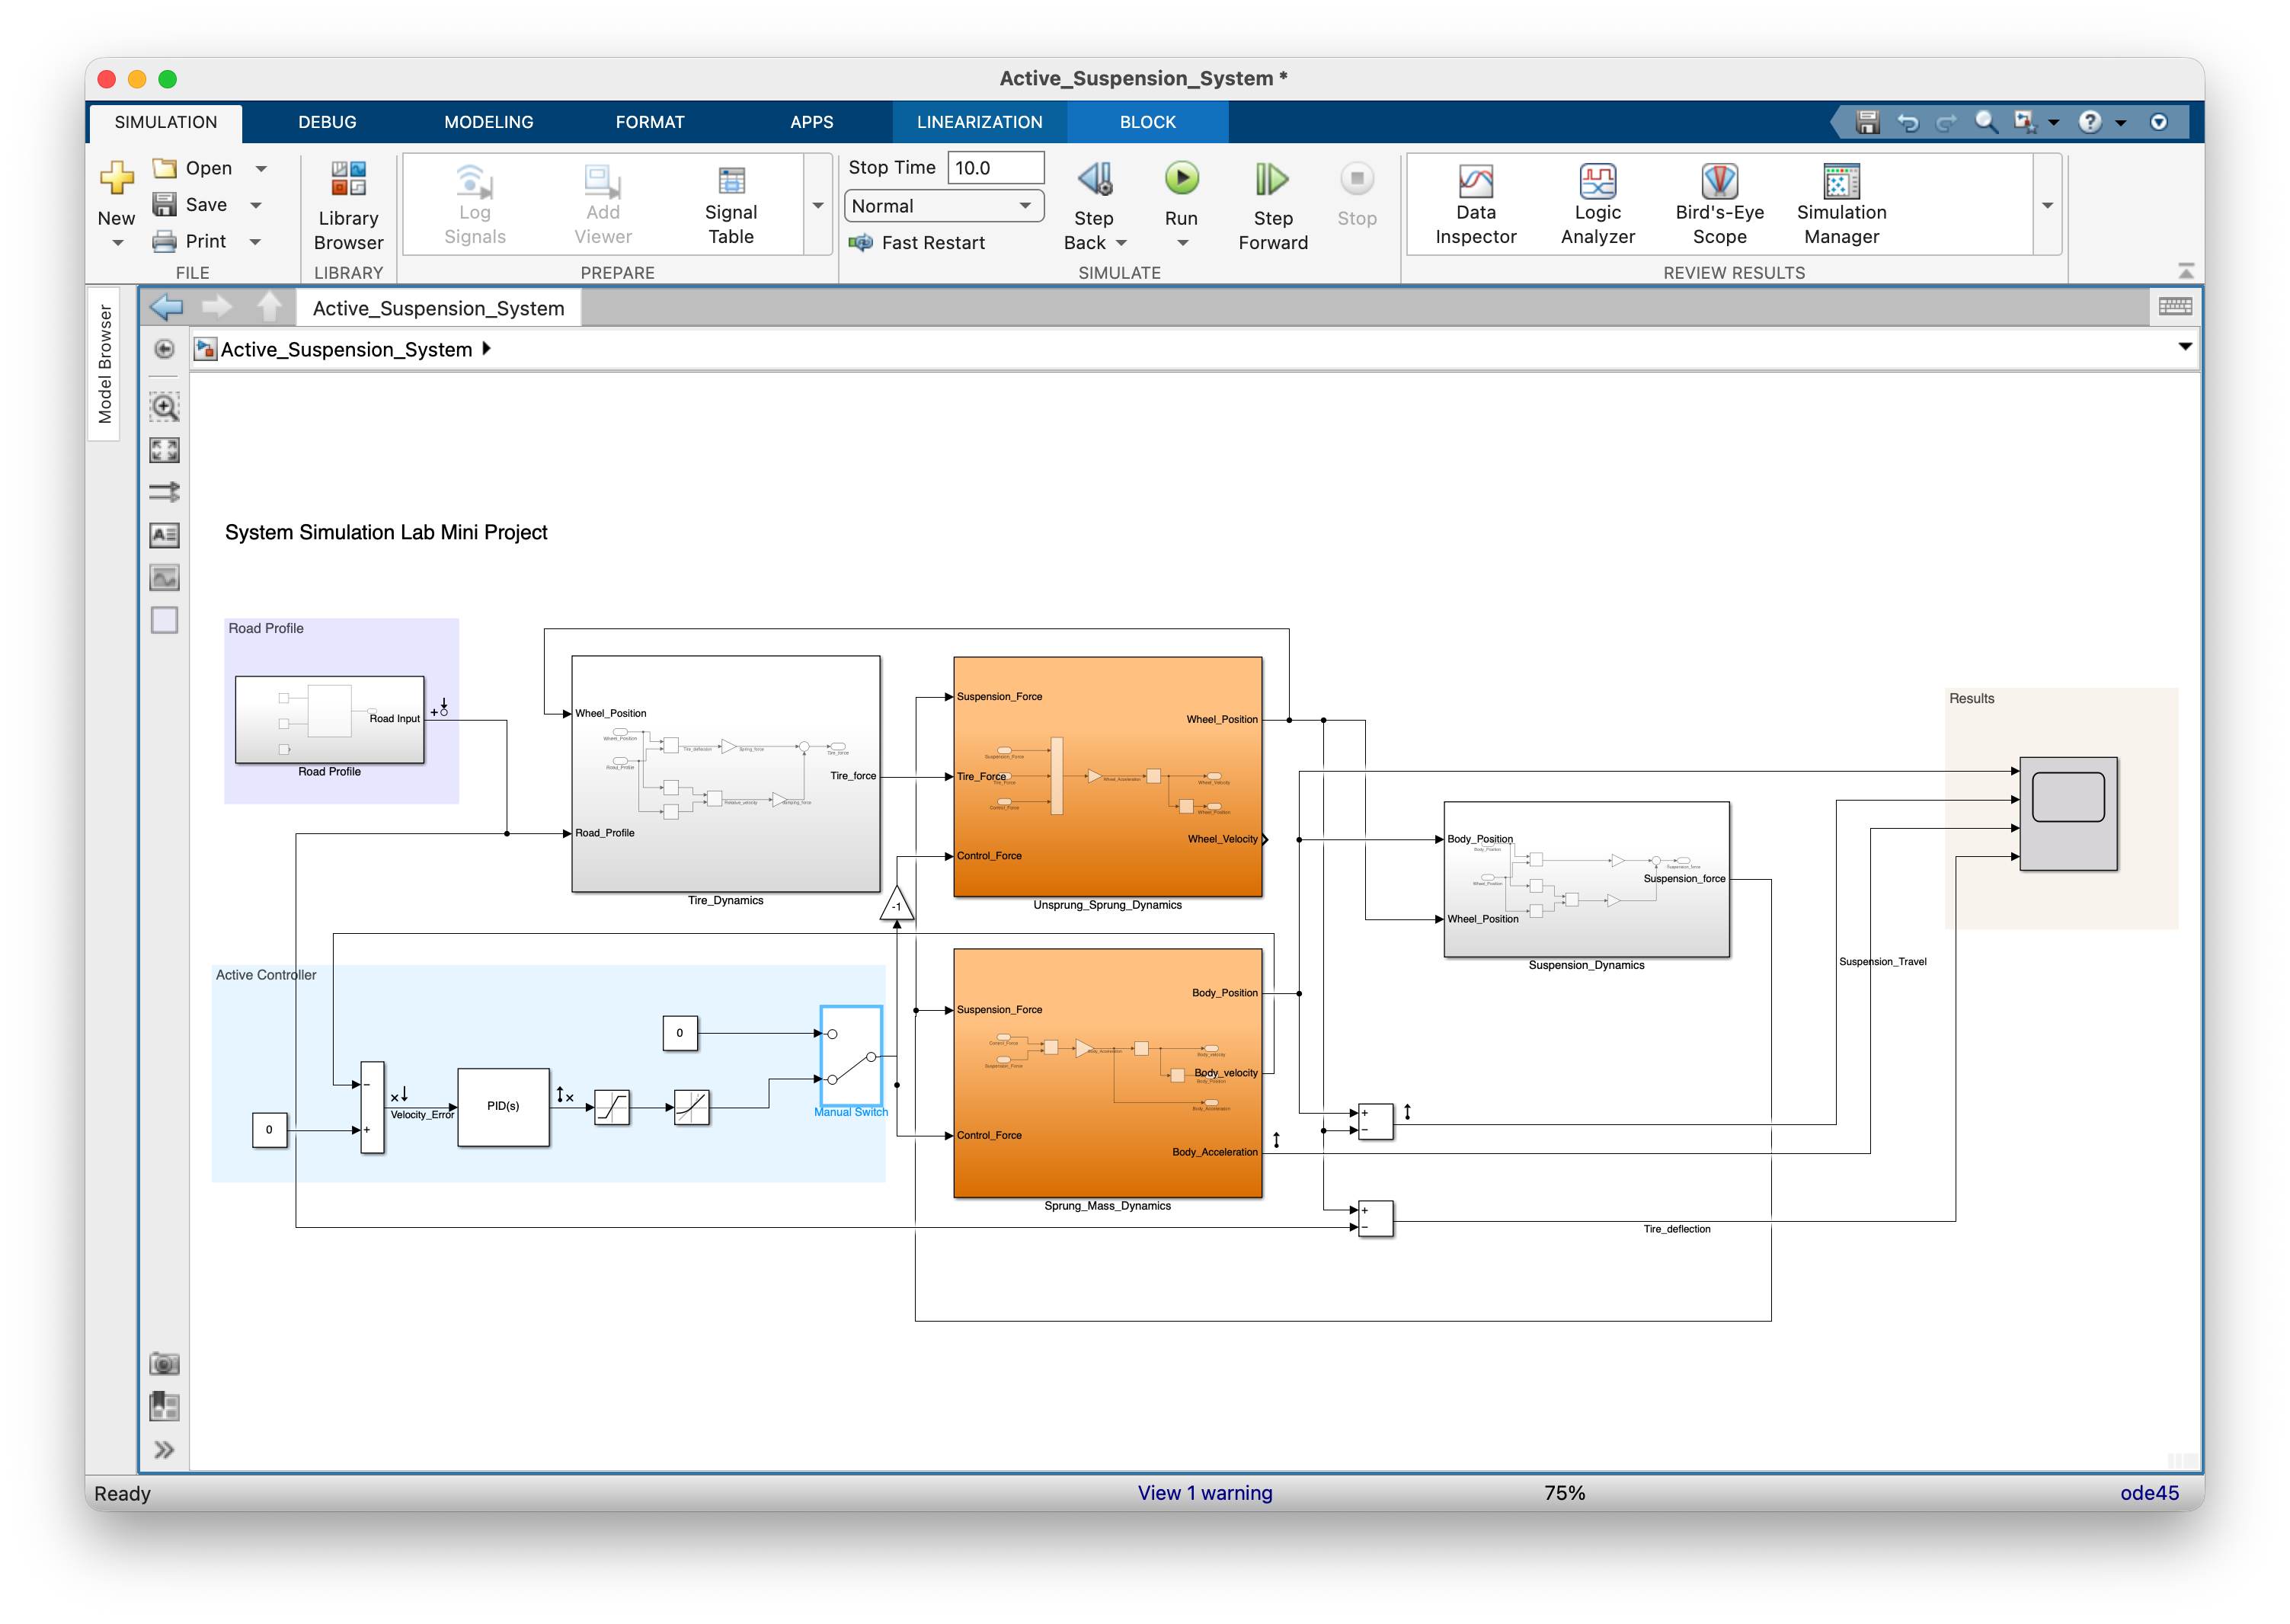
\includegraphics[width=0.95\textwidth,height=0.7\textheight,keepaspectratio]{simulink_screenshot.png}
    \caption{Our complete Simulink implementation}
  \end{figure}
  
\end{frame}

\begin{frame}{Passive System Response}
  \begin{figure}
    \centering
    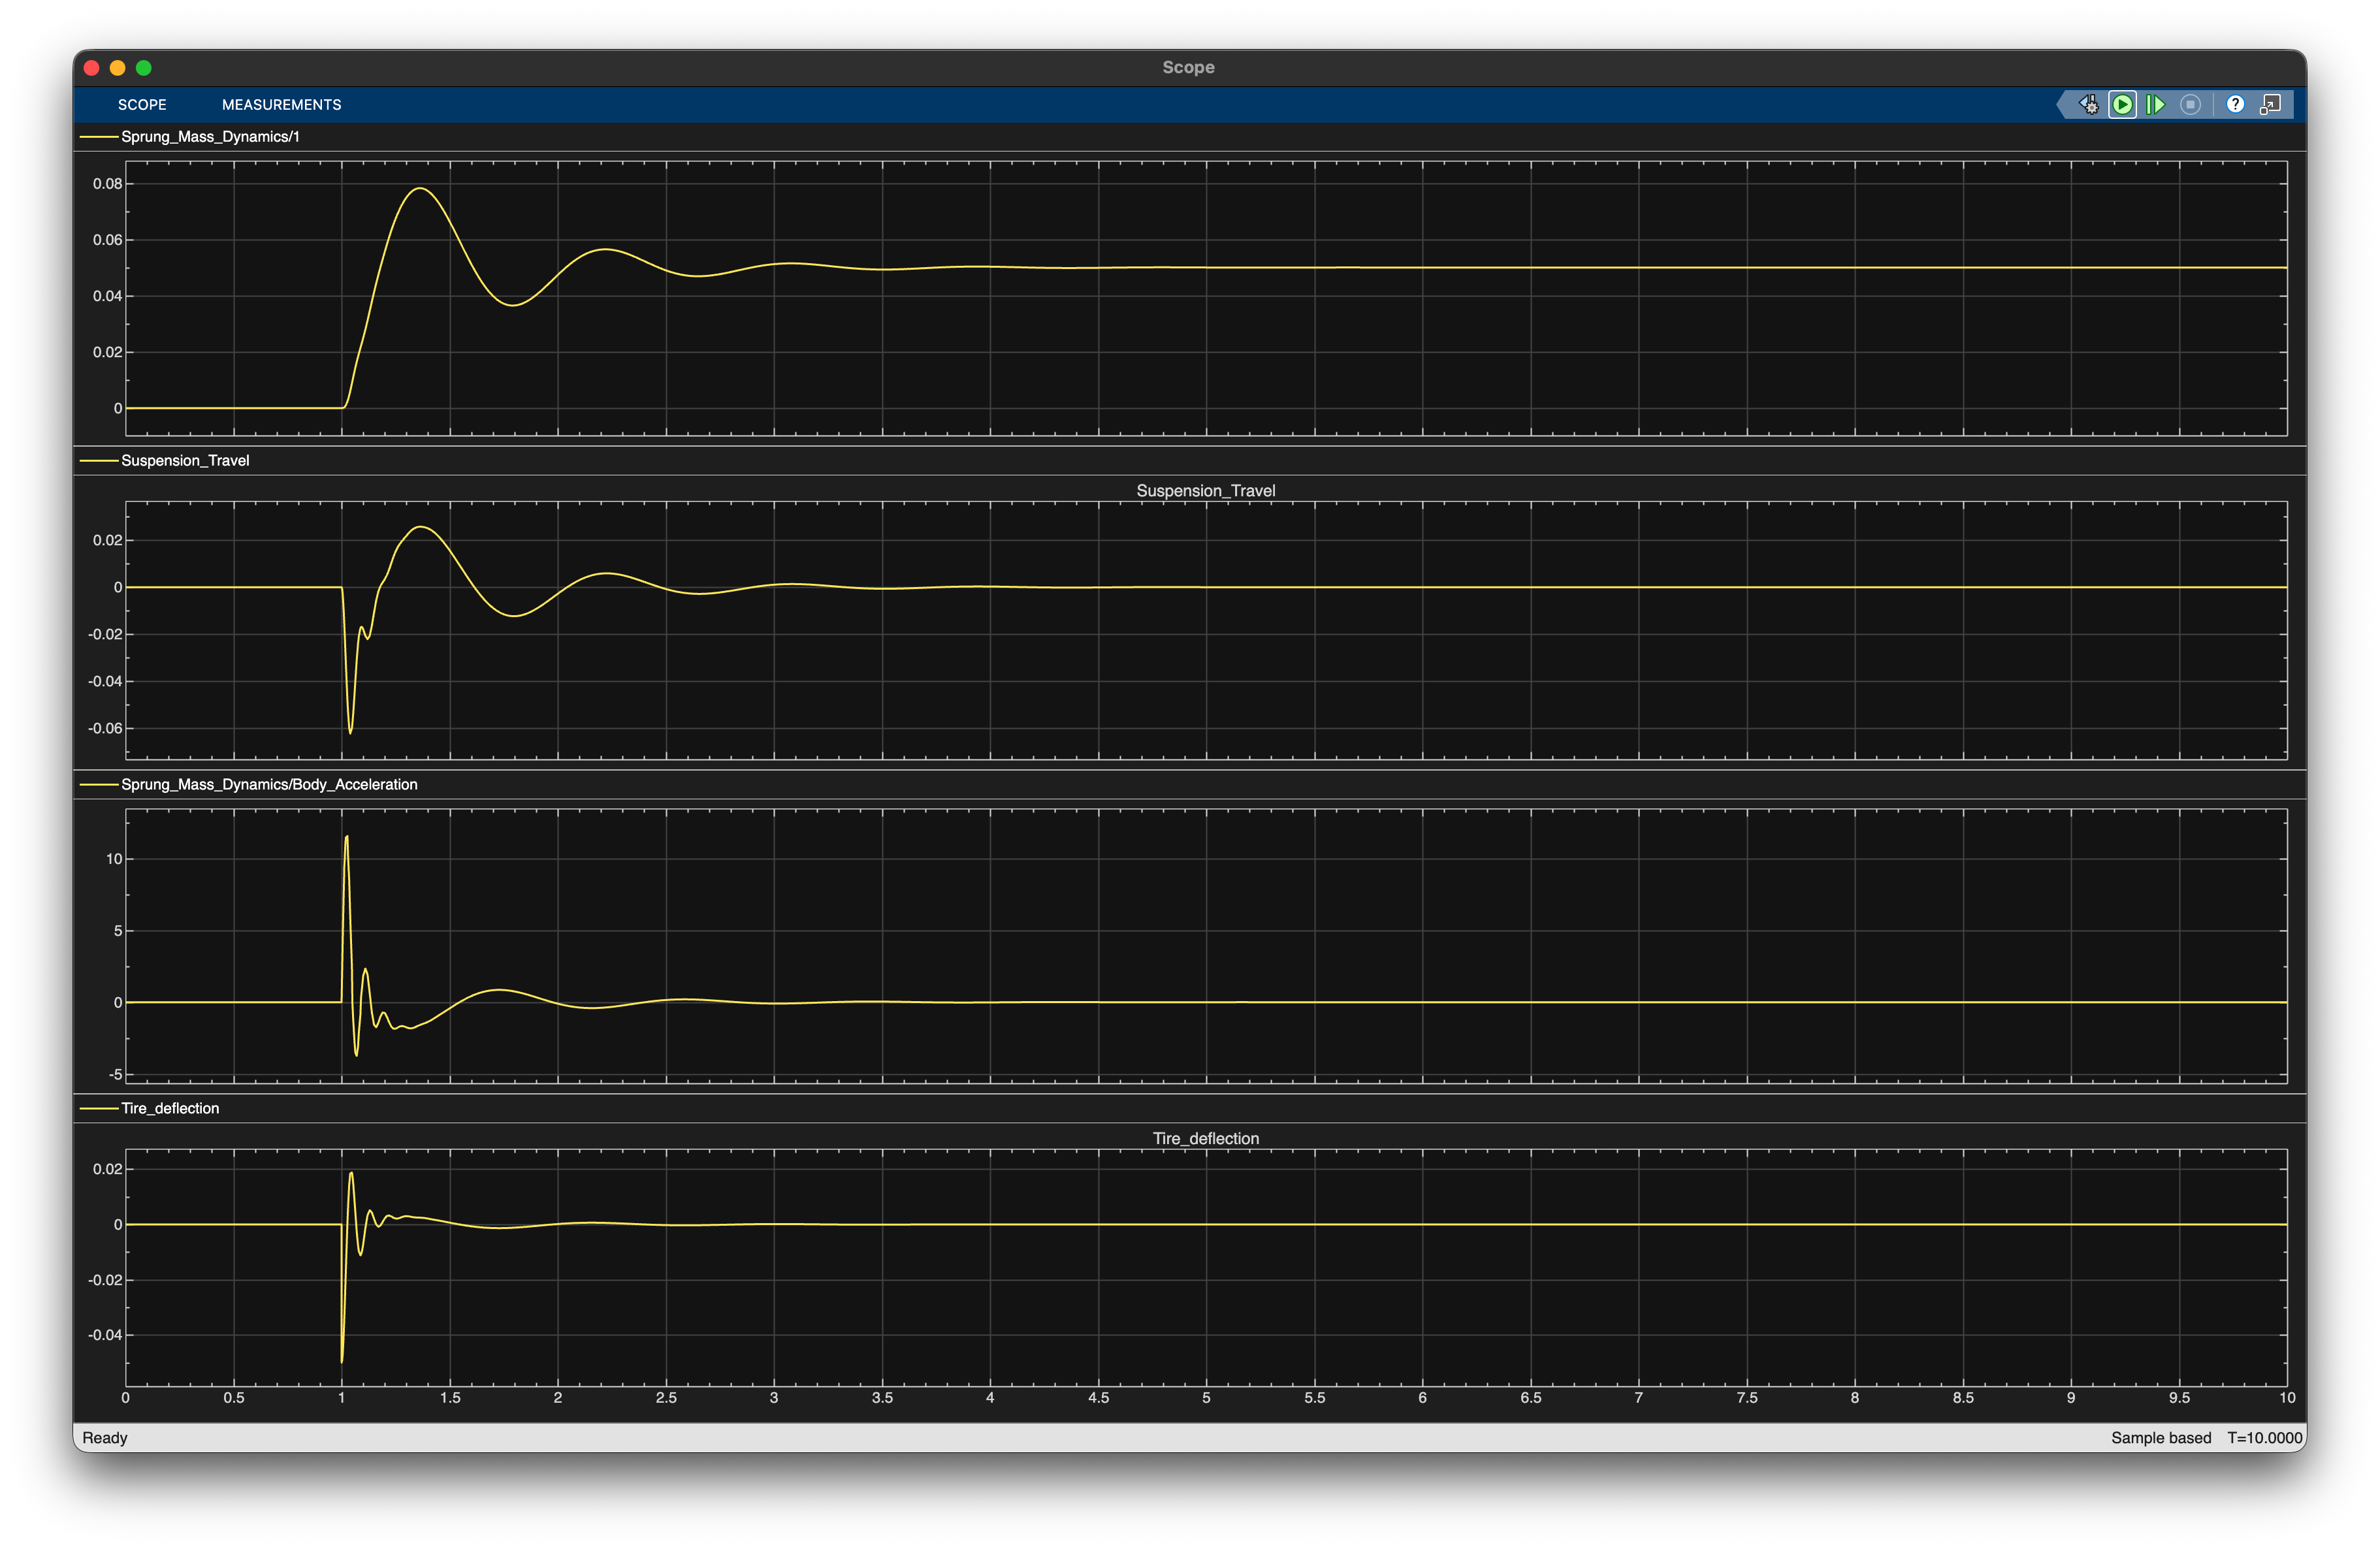
\includegraphics[width=\textwidth,height=0.75\textheight,keepaspectratio]{without_controller.png}
    \caption{Without control - lots of oscillation, peak acceleration = 12 m/s²}
  \end{figure}
\end{frame}

\begin{frame}{Active System Response}
  \begin{figure}
    \centering
    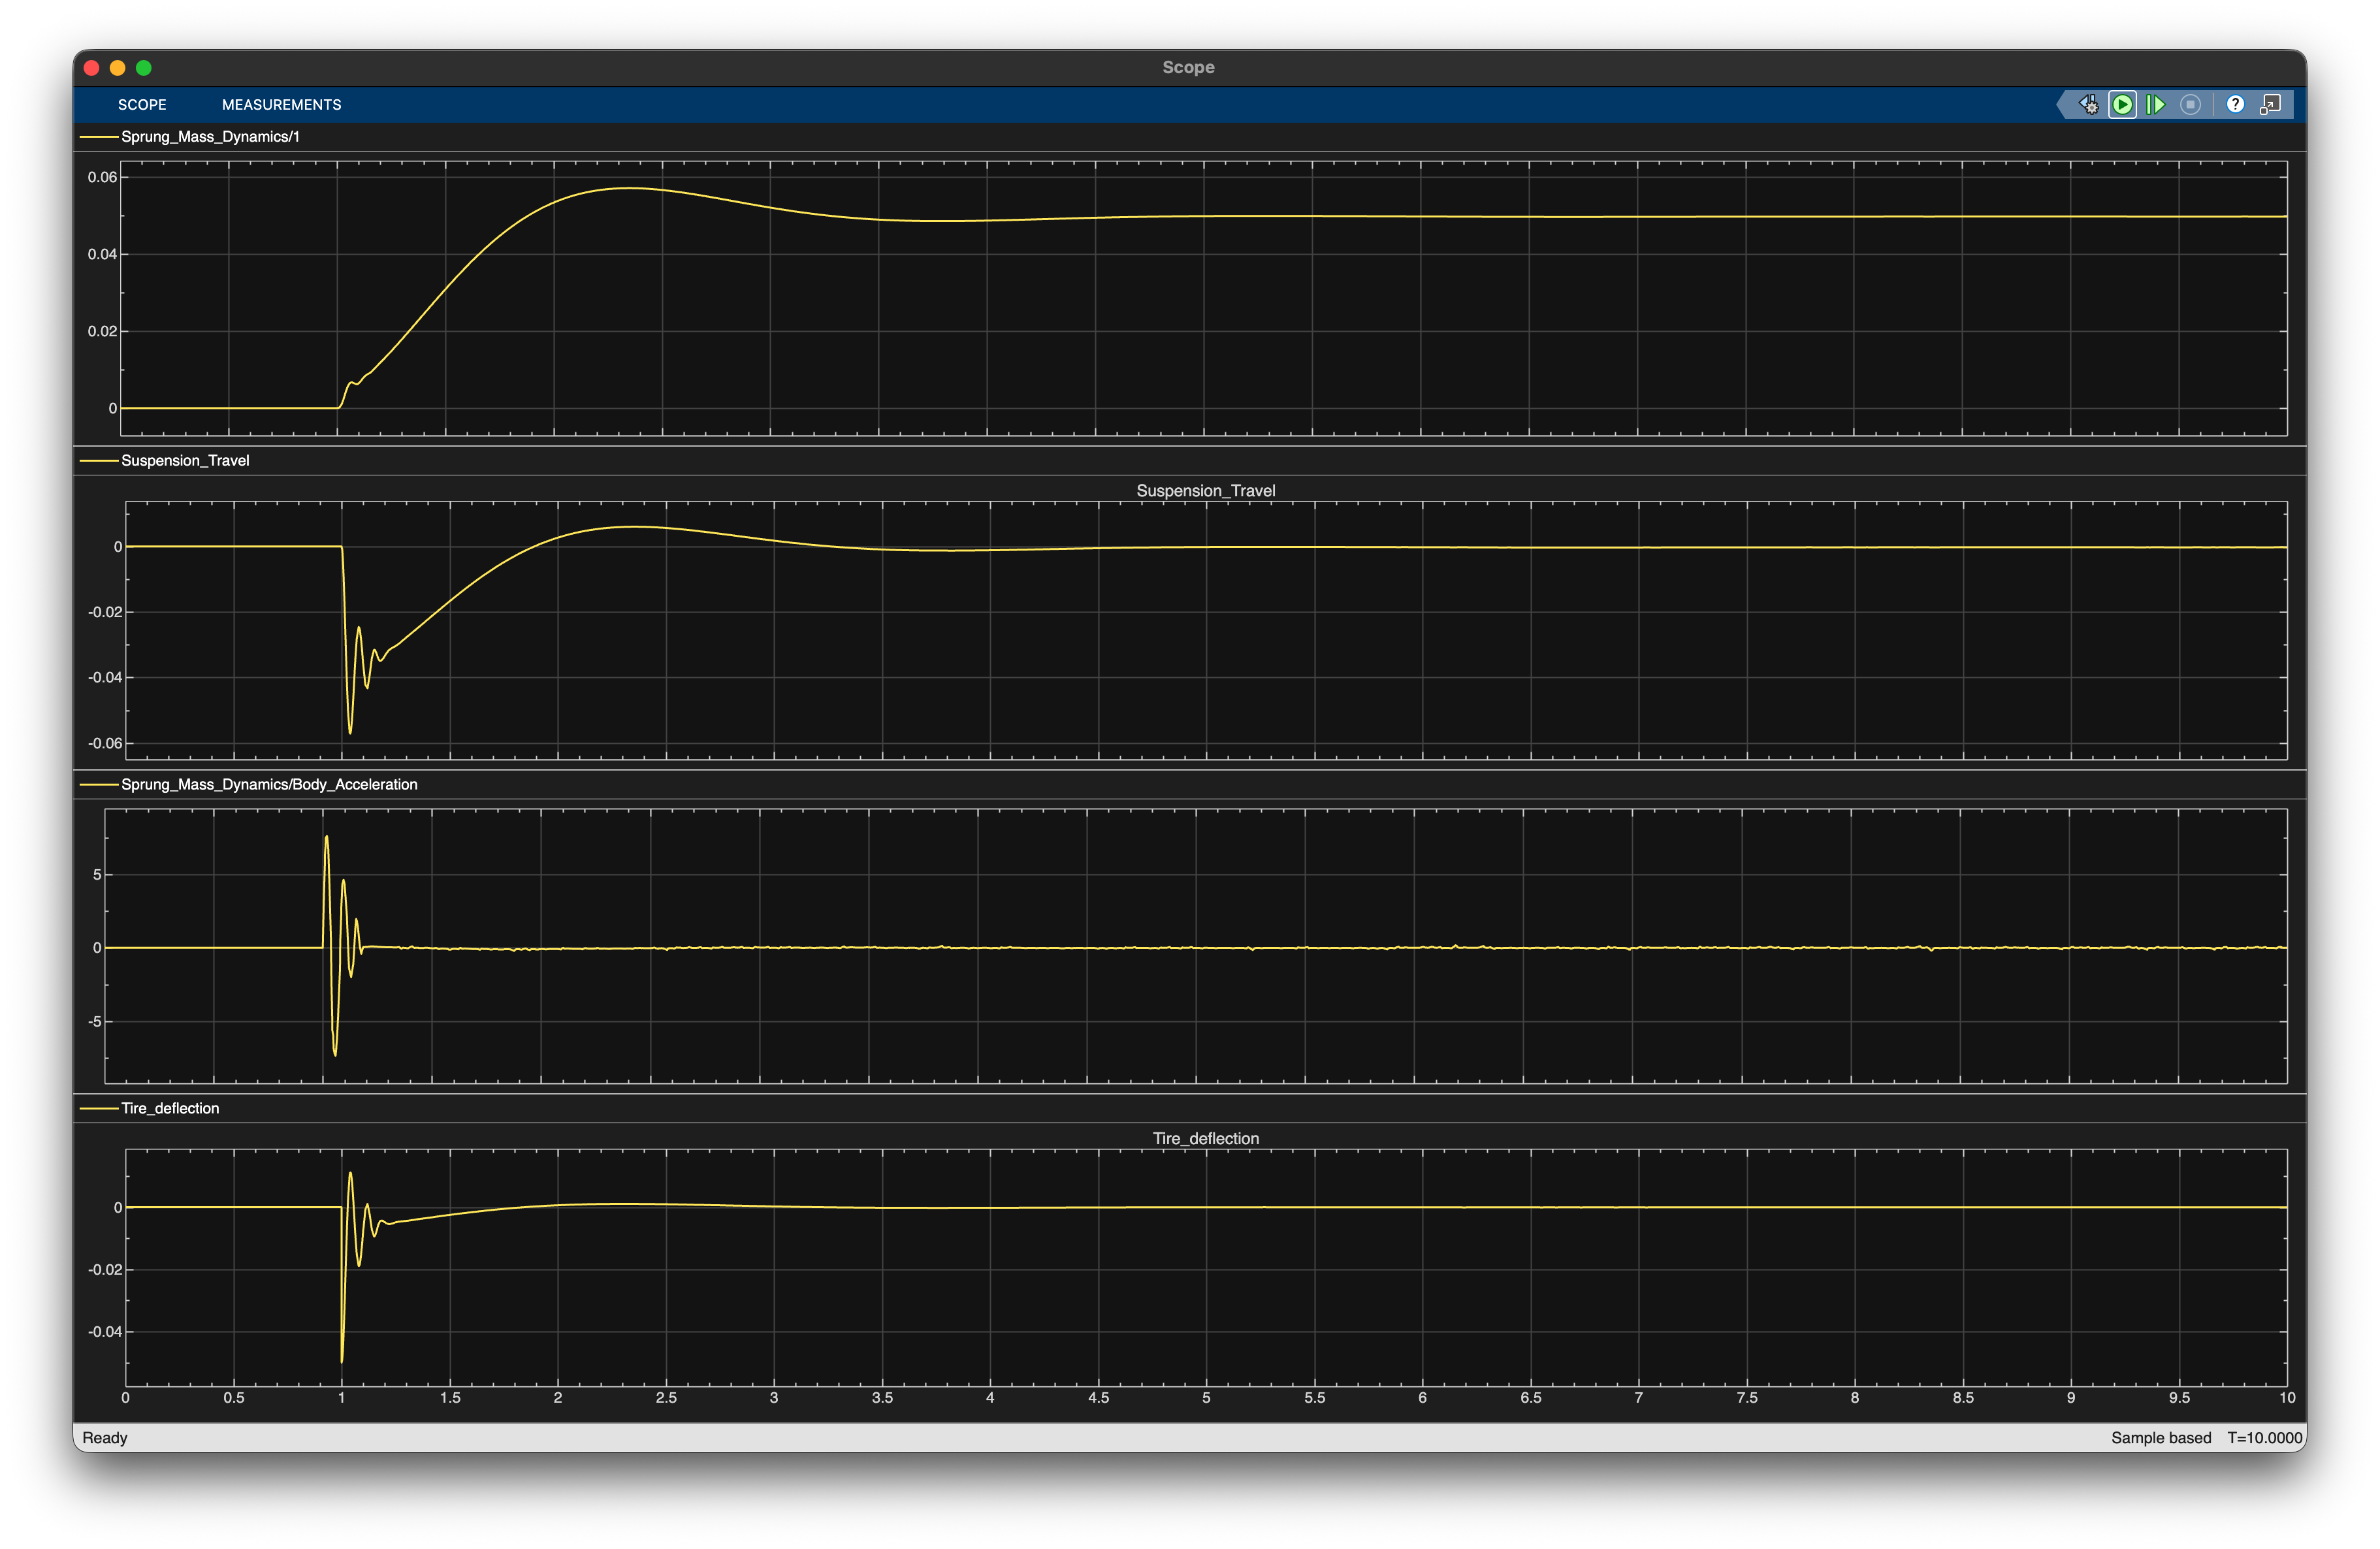
\includegraphics[width=\textwidth,height=0.75\textheight,keepaspectratio]{with_controller.png}
    \caption{With our PID controller - much better! Peak acceleration = 6 m/s²}
  \end{figure}
\end{frame}

\begin{frame}{Comparison of Results}
  \begin{table}
    \centering
    \small
    \begin{tabular}{lccc}
      \toprule
      \textbf{What We Measured} & \textbf{Passive} & \textbf{Active} & \textbf{How Much Better} \\
      \midrule
      Peak acceleration (m/s²) & 12.0 & 6.0 & \textcolor{red}{50\% ↓} \\
      Settling time (s) & 4.0 & 1.5 & \textcolor{red}{62.5\% ↓} \\
      Suspension travel (m) & 0.08 & 0.05 & \textcolor{red}{37.5\% ↓} \\
      Overshoot (\%) & 43.6 & 4.3 & \textcolor{red}{90\% ↓} \\
      Damping ratio & 0.258 & 0.688 & \textcolor{red}{166\% ↑} \\
      \midrule
      Peak magnitude (dB) & 5.98 & -9.26 & \textcolor{red}{15.24 dB ↓} \\
      Vibration reduction & -- & -- & \textcolor{red}{82.7\%} \\
      \bottomrule
    \end{tabular}
  \end{table}
  
  Pretty significant improvements across the board!
\end{frame}

\begin{frame}{How Does It Actually Work?}
  \textbf{What's happening inside:}
  
  \begin{enumerate}
    \item Our PID controller watches the body velocity all the time
    \item When it sees the car body moving up → it pushes down
    \item When it sees the body moving down → it pushes up
    \item This creates "active damping" without wasting energy like regular dampers
    \item The integral part makes sure there's no leftover error
    \item The derivative part predicts what's coming next
  \end{enumerate}
  
  \vspace{0.4cm}
  
  \begin{columns}
    \column{0.5\textwidth}
    \textbf{Why it's better:}
    \begin{itemize}
      \item 82.7\% less vibration
      \item 62.5\% faster response
      \item Better handling
      \item Can adapt
    \end{itemize}
    
    \column{0.5\textwidth}
    \textbf{The downsides:}
    \begin{itemize}
      \item More complex
      \item Needs power
      \item More expensive
      \item More maintenance
    \end{itemize}
  \end{columns}
\end{frame}

% Section: Conclusions
\section{What We Learned}

\begin{frame}{Our Main Findings}
  \begin{block}{What we accomplished:}
    \begin{enumerate}
      \item Built a complete mathematical model with transfer functions
      \item Designed a PID controller and figured out why the gains work
      \item Got 82.7\% reduction in vibrations (that 15.24 dB improvement)
      \item Cut peak acceleration in half (12 → 6 m/s²)
      \item Made settling time 62.5\% faster (4 → 1.5 s)
      \item Improved damping ratio by 166\% (0.258 → 0.688)
      \item Everything checked out in our simulations
    \end{enumerate}
  \end{block}
  
  \vspace{0.3cm}
  
  \begin{alertblock}{Bottom Line}
    Active suspension with PID control is WAY better than passive suspension. We proved it mathematically and through simulation!
  \end{alertblock}
\end{frame}

\begin{frame}{Challenges We Faced}
  \textbf{Things that were tricky:}
  
  \begin{itemize}
    \item Getting the transfer function derivation right took a while - lots of algebra!
    \item Tuning the PID gains was iterative - had to try different values
    \item Making sure the system stayed stable with our chosen gains
    \item Understanding why we got that specific 15.24 dB improvement
    \item Simulink implementation had some bugs initially
  \end{itemize}
  
  \vspace{0.5cm}
  
  \textbf{What helped:}
  \begin{itemize}
    \item Breaking down the problem step by step
    \item Testing one thing at a time
    \item Comparing our calculated values with simulation results
    \item Using MATLAB for all the numerical calculations
  \end{itemize}
\end{frame}

% References
\begin{frame}{References}
  \footnotesize
  \begin{enumerate}
    \item Norman S. Nise, \textit{Control Systems Engineering}, 8th Edition, Wiley, 2019
    \item Katsuhiko Ogata, \textit{Modern Control Engineering}, 5th Edition, Prentice Hall, 2010
    \item Rajesh Rajamani, \textit{Vehicle Dynamics and Control}, 2nd Edition, Springer, 2012
    \item MATLAB Documentation, \textit{Control System Toolbox}, MathWorks, 2025
    \item D. Hrovat, "Survey of Advanced Suspension Developments," \textit{Automatica}, 1997
    \item Laboratory Manual, \textit{Systems Simulation Laboratory ELE 3142}, MIT, 2025
  \end{enumerate}
\end{frame}

% Thank You Slide
\begin{frame}[plain]
  \begin{center}
    \Huge{\textcolor{mitblue}{\textbf{Thank You!}}}
    
    \vspace{1cm}
    
    \Large{Questions?}
    
    \vspace{1.5cm}
    
    \normalsize
    \textbf{Gonugondla Veera Manikanta (230906450)} \\
    \textbf{Rounak Pradhan (230906492)}
    
    \vspace{0.5cm}
    
    Systems Simulation Laboratory (ELE 3142) \\
    Department of Electrical \& Electronics Engineering \\
    Manipal Institute of Technology
  \end{center}
\end{frame}

\end{document}